\documentclass[a4paper,11pt]{article}

\usepackage[ngerman]{babel}
\usepackage[utf8]{inputenc}
\usepackage[T1]{fontenc}
\usepackage{geometry}
\geometry{left=25mm,right=25mm,top=25mm,bottom=25mm}
\usepackage{graphicx}
\usepackage{url}
\usepackage{parskip}

\begin{document}
	
	\begin{center}
		{\LARGE \textbf{Kurzanleitung Ultraschallradar}}\\[0.5em]
		{\large (Ultraschall-Radarsystem mit Benutzeroberfläche auf PC)}
	\end{center}
	
	\vspace{1em}
	
	% Optionales Übersichtsbild
	\begin{figure}[h]
		\centering
		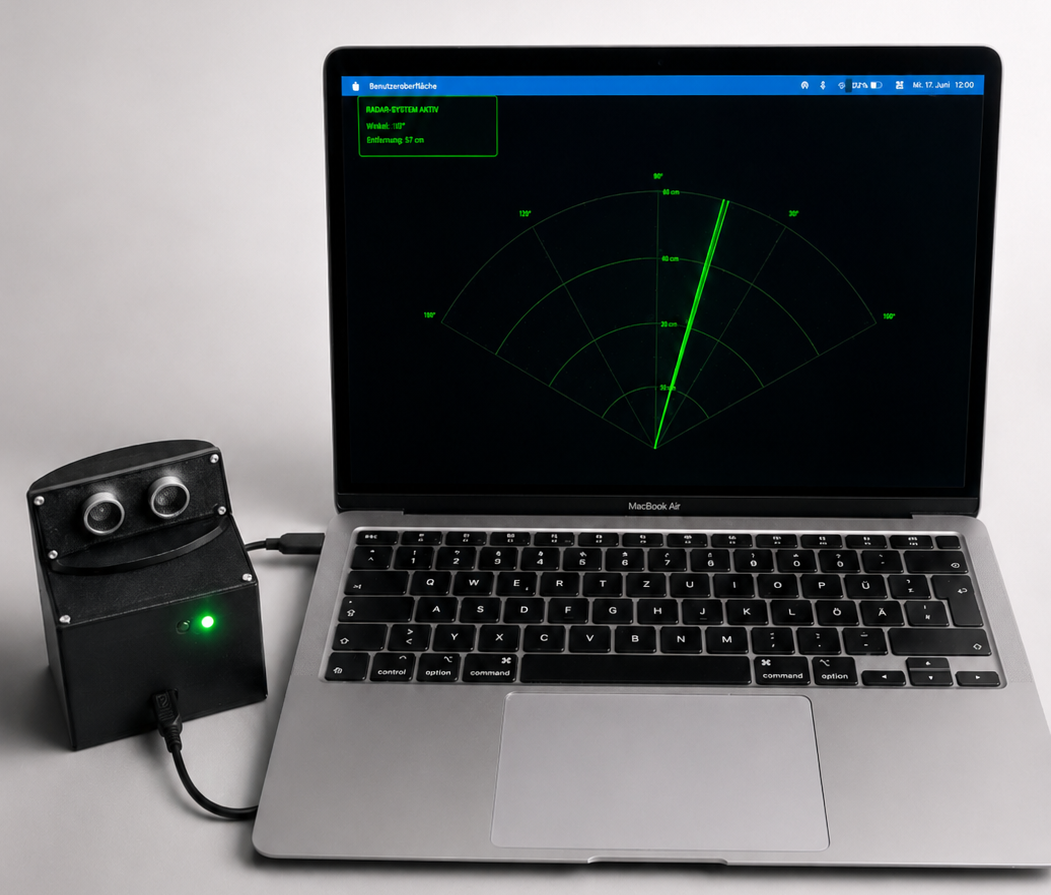
\includegraphics[width=0.7\textwidth]{../Manuals/Benutzerhandbuch/Bilder/GesamtsystemUltraschallradar.png}
		\caption{Gesamtsystem Ultraschallradar}
	\end{figure}
	
	\section{Einleitung}
	
	Diese Kurzanleitung beschreibt die wichtigsten Schritte, um das Ultraschall-Radarsystem sicher zu starten und zu bedienen.
	Das Radarsystem ist fertig montiert, es sind nur wenige Handgriffe nötig.
	
	\section{Sicherheitshinweise}
	
	\textbf{Bewegliche Teile:} Während des Betriebs nicht in die Dreheinheit greifen, sonst können Kabel oder Mechanik beschädigt werden. 
	
	\begin{itemize}
		\item Gerät nur an einem standardkonformen Computer-USB-Ausgang (5\,V) betreiben.
		\item Gerät von Flüssigkeiten fernhalten.
	\end{itemize}
	
	\section{Inbetriebnahme}
	
	\subsection{Aufstellung}
	
	Radarsystem auf eine ebene Fläche (z.\,B. Tisch) stellen und dafür sorgen , dass keine Gegenstände die Rotation der Dreheinheit behindern. 
	
	\subsection{Software vom USB-Stick starten}
	
	Die PC-Software zur Visualisierung liegt auf dem mitgelieferten USB-Stick. 
	
	\begin{enumerate}
		\item USB-Stick in den Computer einstecken.
		\item Ordner \texttt{Ultraschallradar-Benutzeroberflaeche} auf den Computer kopieren (z.\,B. Desktop).
		\item Im kopierten Ordner die Datei \textit{„Ultraschallradar-Benutzeroberflaeche-App“} per Doppelklick starten.
	\end{enumerate}
	
	\subsection{Reihenfolge beim Start}
	
	\begin{enumerate}
		\item \textbf{Hardware anschlie\ss en:} Radarsystem über das Micro-USB Kabel mit dem Computer verbinden und Stromversorgung sicherstellen. 
		\item \textbf{Software starten:} Die Benutzeroberfläche wie oben beschrieben aus dem kopierten Ordner starten. 
		\item \textbf{Selbsttest abwarten:} Die Software startet automatisch den Hardware-Selbsttest.
	\end{enumerate}
	
	Während des Selbsttests ist der Bildschirm abgedunkelt, in der Mitte erscheint \textit{„System fährt hoch... Hardware-Selbsttest wird durchgeführt.“}. 
	Die Dreheinheit fährt in die Ausgangsposition (0\(^\circ\)), ein Test-Ultraschallimpuls wird gesendet, und kurz leuchten beide LEDs am Gehäuse (grün und rot). 
	Währenddessen sind keine Eingaben erforderlich.
	\newpage
	
	\section{Bedienung und Anzeige}
	
	\subsection{Radarbild}
	
	Nach bestandenem Selbsttest wechselt das System in den Normalbetrieb, die grüne Status-LED leuchtet dauerhaft. 
	Auf dem Bildschirm erscheint eine kreisförmige Anzeige mit Radar-Gitter und einem Scan-Strahl, der von 30\(^\circ\) bis 150\(^\circ\) und zurück läuft. 
	Erkannte Hindernisse werden je nach Größe als rote Punkte oder Linien auf dem Gitter dargestellt. 
	
	\subsection{Reichweite und Statusanzeige}
	
	In der oberen linken Ecke zeigt die Statusanzeige den Systemzustand („SYSTEM OK“), den aktuellen Scan-Winkel und die Distanz zum nächsten Objekt in Zentimetern. 
	Das System erkennt Objekte zuverlässig in einem Bereich von etwa 2\,cm bis 40\,cm. Über die 40\,cm hinaus erkennt das System auch noch Objekte, kann diese aber nicht mehr visuell in der grafischen Benutzeroberfläche darstellen.
	
	\section{Fehlermeldungen und Fehlersuche}
	
	\subsection{Software-Fehlermeldung}
	
	Tritt während Selbsttest oder Betrieb ein kritischer Hardwarefehler auf, werden alle Servobewegungen sofort gestoppt. 
	Die Benutzeroberfläche wechselt auf einen roten Warnhintergrund, das Radarbild wird ausgeblendet und folgende Meldung erscheint: 
	
	\begin{quote}
		\textit{„SYSTEMFEHLER – Sicherstellen, dass der Computer mit dem Radarsystem verbunden ist! – Anlage überprüfen und neustarten.“}
	\end{quote}
	
	Am Gehäuse leuchtet die rote LED dauerhaft. 
	
	\subsection{Vorgehen bei Systemfehler}
	
	\begin{enumerate}
		\item Radarsystem stromlos machen (USB-Kabel zum Computer trennen). 
		\item Prüfen, ob der Ultraschallsensor beim Start nicht durch ein Objekt direkt vor der Front (0\,cm) blockiert wird. 
		\item USB-Verbindung wiederherstellen und die Benutzeroberfläche neu starten, damit der Selbsttest erneut ausgeführt wird. 
	\end{enumerate}
	
\end{document}